% =====================================================================
% Figure: Method-positioning RADAR (spider) chart -- AEGIS vs the two prior
% threads it unifies (structural attacks; certifiers). Honest variant of the
% capability matrix (fig_positioning): axes are scored on [0,1] (0 = centre,
% 1 = outer ring) and DELIBERATELY include axes where rivals win, so no method
% fills the whole space (defuses the strawman concern, editorial item C-DA2).
%
% Score rationale (all defensible from the paper / related work):
%   Attack direction      AEGIS 1.0 (closed-form SVD, prop:attack) | Attacks 0.9
%                         (their core function) | Certifiers 0.0
%   Per-edge attribution  AEGIS 1.0 (||[S_c]_{:,k}||) | Attacks 0.8 (greedy/grad
%                         edge selection) | Certifiers 0.0 (do not name edges)
%   Large-budget damage   Attacks 1.0 (GR-BCD/PR-BCD dominate at large budgets) |
%                         AEGIS 0.5 (one-query early-warning regime) | Cert. 0.0
%   Per-node certificate  Certifiers 1.0 (sound prob./determ. radii) | AEGIS 0.65
%                         (first-order r_v + conformal under exchangeability) | Atk 0.0
%   Label-free/no-retrain AEGIS 1.0 | Certifiers 0.85 (sampling, no labels) |
%                         Attacks 0.35 (poisoning needs labels/surrogate)
%   Query efficiency      AEGIS 1.0 (one query) | Attacks 0.3 (50-step/512-query) |
%                         Certifiers 0.1 (1e3-1e4 MC samples/node)
% Okabe-Ito palette, mathptmx serif 11pt: consistent with the other figures.
% =====================================================================
\documentclass[tikz,border=6pt,11pt]{standalone}
\usepackage[T1]{fontenc}
\usepackage{mathptmx}
\usepackage{tikz}
\usetikzlibrary{calc}
\usepackage{xcolor}
\usepackage{amsmath,amssymb}
\usepackage{xspace}
\newcommand{\AEGIS}{\textsc{Aegis}\xspace}
\renewcommand{\familydefault}{\rmdefault}

% Okabe-Ito (colourblind-safe; shared with the other paper figures)
\definecolor{okBlue}{HTML}{0072B2}
\definecolor{okOrange}{HTML}{E69F00}
\definecolor{okGreen}{HTML}{009E73}
\definecolor{okVermilion}{HTML}{D55E00}
\definecolor{okGrey}{HTML}{888888}

\begin{document}
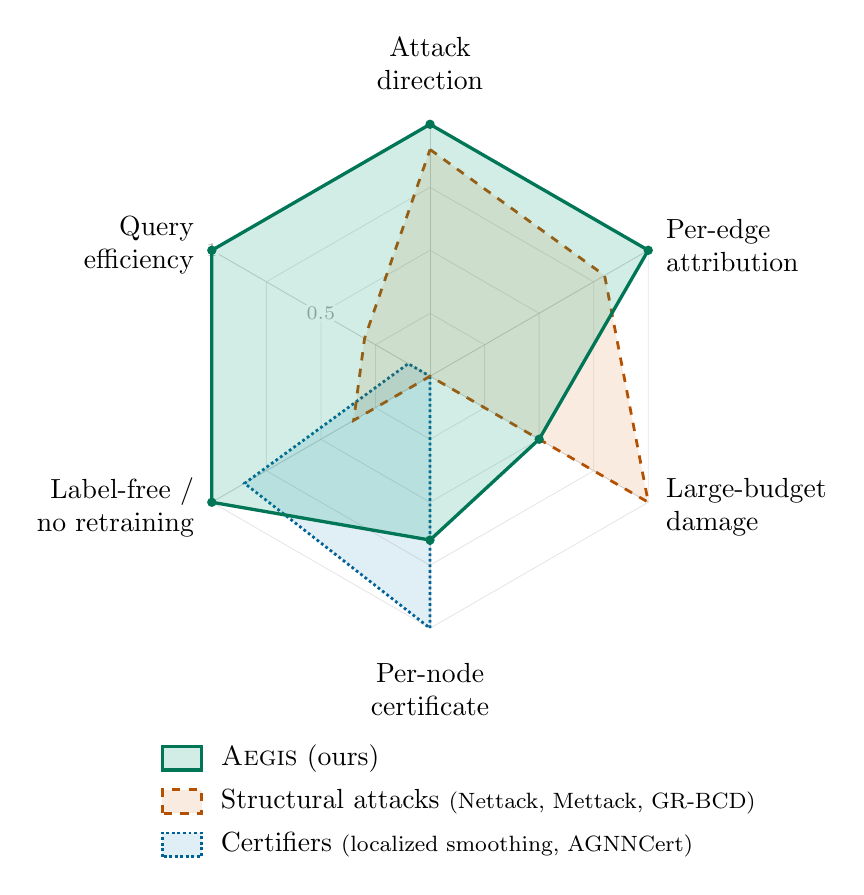
\begin{tikzpicture}[font=\rmfamily]

% --- concentric grid rings (hexagons at r = 0.25,0.5,0.75,1.0 of R=3.2) ------
\foreach \rr in {0.8,1.6,2.4,3.2}{
  \draw[okGrey!22, line width=0.3pt]
    (90:\rr)--(30:\rr)--(-30:\rr)--(-90:\rr)--(-150:\rr)--(150:\rr)--cycle;
}
% --- radial spokes -----------------------------------------------------------
\foreach \a in {90,30,-30,-90,-150,150}{
  \draw[okGrey!38, line width=0.3pt] (0,0)--(\a:3.2);
}
% scale hint: 1 at the outer ring on the upper-left (least busy) spoke
\node[okGrey!75, font=\scriptsize, fill=white, inner sep=0.6pt] at (150:1.6) {$0.5$};
\node[okGrey!75, font=\scriptsize, fill=white, inner sep=0.6pt] at (150:3.2) {$1$};

% --- polygons (drawn behind to front: Certifiers, Attacks, AEGIS) ------------
% Certifiers: certificate 1.0, label-free 0.85, efficiency 0.1; rest 0
\draw[okBlue!85!black, line width=1.0pt, densely dotted, fill=okBlue, fill opacity=0.12]
  (90:0)--(30:0)--(-30:0)--(-90:3.2)--(-150:2.72)--(150:0.32)--cycle;
% Structural attacks: attack-dir 0.9, per-edge 0.8, large-budget 1.0,
% certificate 0.0, label-free 0.35, efficiency 0.3
\draw[okVermilion!85!black, line width=1.0pt, dashed, fill=okVermilion, fill opacity=0.12]
  (90:2.88)--(30:2.56)--(-30:3.2)--(-90:0)--(-150:1.12)--(150:0.96)--cycle;
% AEGIS: attack-dir 1.0, per-edge 1.0, large-budget 0.5, certificate 0.65,
% label-free 1.0, efficiency 1.0
\draw[okGreen!75!black, line width=1.2pt, fill=okGreen, fill opacity=0.18]
  (90:3.2)--(30:3.2)--(-30:1.6)--(-90:2.08)--(-150:3.2)--(150:3.2)--cycle;
% AEGIS vertex markers (it is the only method with mass on every axis)
\foreach \a/\r in {90/3.2, 30/3.2, -30/1.6, -90/2.08, -150/3.2, 150/3.2}{
  \fill[okGreen!75!black] (\a:\r) circle (1.7pt);
}

% --- axis labels -------------------------------------------------------------
\node[anchor=south, align=center]            at (90:3.52)  {Attack\\direction};
\node[anchor=west,  align=left]              at (30:3.32)  {Per-edge\\attribution};
\node[anchor=west,  align=left]              at (-30:3.32) {Large-budget\\damage};
\node[anchor=north, align=center]            at (-90:3.52) {Per-node\\certificate};
\node[anchor=east,  align=right]             at (-150:3.32){Label-free /\\no retraining};
\node[anchor=east,  align=right]             at (150:3.32) {Query\\efficiency};

% --- legend (below the chart) ------------------------------------------------
\begin{scope}[shift={(0,-5.0)}]
  \def\sw{0.5}     % swatch width
  \draw[okGreen!75!black, line width=1.2pt, fill=okGreen, fill opacity=0.18]
    (-3.4,0) rectangle ++(\sw,0.30);
  \node[anchor=west] at (-3.4+\sw+0.12, 0.15) {\AEGIS\ (ours)};
  \draw[okVermilion!85!black, line width=1.0pt, dashed, fill=okVermilion, fill opacity=0.12]
    (-3.4,-0.55) rectangle ++(\sw,0.30);
  \node[anchor=west] at (-3.4+\sw+0.12, -0.40)
    {Structural attacks \textnormal{\footnotesize(Nettack, Mettack, GR-BCD)}};
  \draw[okBlue!85!black, line width=1.0pt, densely dotted, fill=okBlue, fill opacity=0.12]
    (-3.4,-1.10) rectangle ++(\sw,0.30);
  \node[anchor=west] at (-3.4+\sw+0.12, -0.95)
    {Certifiers \textnormal{\footnotesize(localized smoothing, AGNNCert)}};
\end{scope}

\end{tikzpicture}
\end{document}
